%%%%%%%%%%%%%%%%%%%%%%%%%%%%%%%%%%%%%%%%%
% Uppsala University Assignment Title Page 
% LaTeX Template
% Version 1.0 (27/12/12)
%
% This template has been downloaded from:
% http://www.LaTeXTemplates.com
%
% Original author:
% WikiBooks (http://en.wikibooks.org/wiki/LaTeX/Title_Creation)
% Modified by Elsa Slattegard to fit Uppsala university
% License:
% CC BY-NC-SA 3.0 (http://creativecommons.org/licenses/by-nc-sa/3.0/)

%\title{Title page with logo}
%----------------------------------------------------------------------------------------
%	PACKAGES AND OTHER DOCUMENT CONFIGURATIONS
%----------------------------------------------------------------------------------------

\documentclass[12pt]{article}
\usepackage[english]{babel}
\usepackage[utf8x]{inputenc}
\usepackage{amsmath}
\usepackage{amssymb}
\usepackage{dsfont}
\usepackage{graphicx}
\usepackage{float}
\usepackage{hyperref}
\usepackage[dvipsnames]{xcolor}
\usepackage[colorinlistoftodos]{todonotes}
\usepackage[ruled,vlined]{algorithm2e}

\setlength {\marginparwidth }{2cm}

\begin{document}
    \begin{titlepage}
    
    \newcommand{\HRule}{\rule{\linewidth}{0.5mm}} % Defines a new command for the horizontal lines, change thickness here
    
    \center % Center everything on the page
     
    %----------------------------------------------------------------------------------------
    %	HEADING SECTIONS
    %----------------------------------------------------------------------------------------
    
    \textsc{\LARGE{T\'{e}cnico Lisboa} \\ \vspace{0.5cm} \LARGE{University of Lisbon}}\\[1cm] % Name of your university/college
    \vspace{-2cm}
    \begin{figure}[H]
        \centering
        \begin{minipage}{.5\textwidth}
            \centering
            \phantom{............}
\includegraphics[width=.9\linewidth]{figures/logos/university-lisbon-logo.png}
        \end{minipage}%
        \begin{minipage}{.5\textwidth}
            \centering
            \hspace{-1cm}
            
\includegraphics[width=.9\linewidth]{figures/logos/tecnico-ulisboa-logo.png}
        \end{minipage}
    \end{figure}
    \vspace{-1cm}
     % Include a department/university logo - this will require the graphicx package
    \textsc{\Large Research Seminar in Information Security}\\[0.5cm] % Major heading such as course name
    \textsc{(Prof. Paulo \uppercase{Mateus})}\\[0.5cm]
    \textsc{Doctoral Program in Information Security}\\[0.5cm] % Minor heading such as course title
    \textsc{\large 2023/2024 - 1\textsuperscript{st} Semester}\\[0.5cm] % Minor heading such as course title
    
    %----------------------------------------------------------------------------------------
    %	TITLE SECTION
    %----------------------------------------------------------------------------------------
    
    \HRule \\[0.3cm]
        { \huge \bfseries Device-Independent Entanglement Certification with Dishonest Parties \\ \vspace{0.5cm} \Large (Gl\'{a}ucia \textsc{\uppercase{Murta}} - November 23, 2023)}\\[0.4cm] % Title of your document
    \HRule \\[1cm]
     
    %----------------------------------------------------------------------------------------
    %	AUTHOR SECTION
    %----------------------------------------------------------------------------------------
    
    \begin{minipage}{0.75\textwidth}
    
        \begin{flushleft} \large
            \textbf{Report written by:}\\
            \begin{itemize}
                \vspace{-0.1cm}
                \item \normalsize{Rúben \textsc{\uppercase{Barreiro}}:\\
                - \href{mailto:ruben.andre.letra.barreiro@tecnico.ulisboa.pt}{\emph{ruben.andre.letra.barreiro@tecnico.ulisboa.pt}}}
            \end{itemize}
        \end{flushleft}
    
    \end{minipage}\\[2cm]
    \vspace{-1cm}    
    % If you don't want a supervisor, uncomment the two lines below and remove the section above
    %\Large \emph{Author:}\\
    %John \textsc{Smith}\\[3cm] % Your name
    
    %----------------------------------------------------------------------------------------
    %	DATE SECTION
    %----------------------------------------------------------------------------------------
    
    {\large{Last updated: \today}}\\[2cm] % Date, change the \today to a set date if you want to be precise
    
    \vfill % Fill the rest of the page with whitespace

    \end{titlepage}

    \clearpage

    
    \section{Motivation}
    \label{sec:motivation}

    One of the tasks of interest in this seminar is to address how to certify some resource states and their quantum properties distributed in a future\break (experimental) Quantum Communication Network connecting several\break quantum devices (or quantum nodes) in different places. These quantum properties can be entanglement properties of those resource states distributed on a Quantum Communication Network involving some scenario aspects, such as geographic proximity or political relations. These quantum nodes might be prone to collaborate with each other, so we cannot assume they do their tasks independently. In these scenarios, we would like to certify the entanglement properties even in the presence of some dishonest party. Here, the minimal level of characterization we would want to guarantee for these quantum network systems is that they are Device-Independent (DI). In this characterization scenario, we assume that there might exist some dishonest parties in the quantum network. However, we also want to keep the privacy
    
    \begin{figure}[ht]
        \centering
        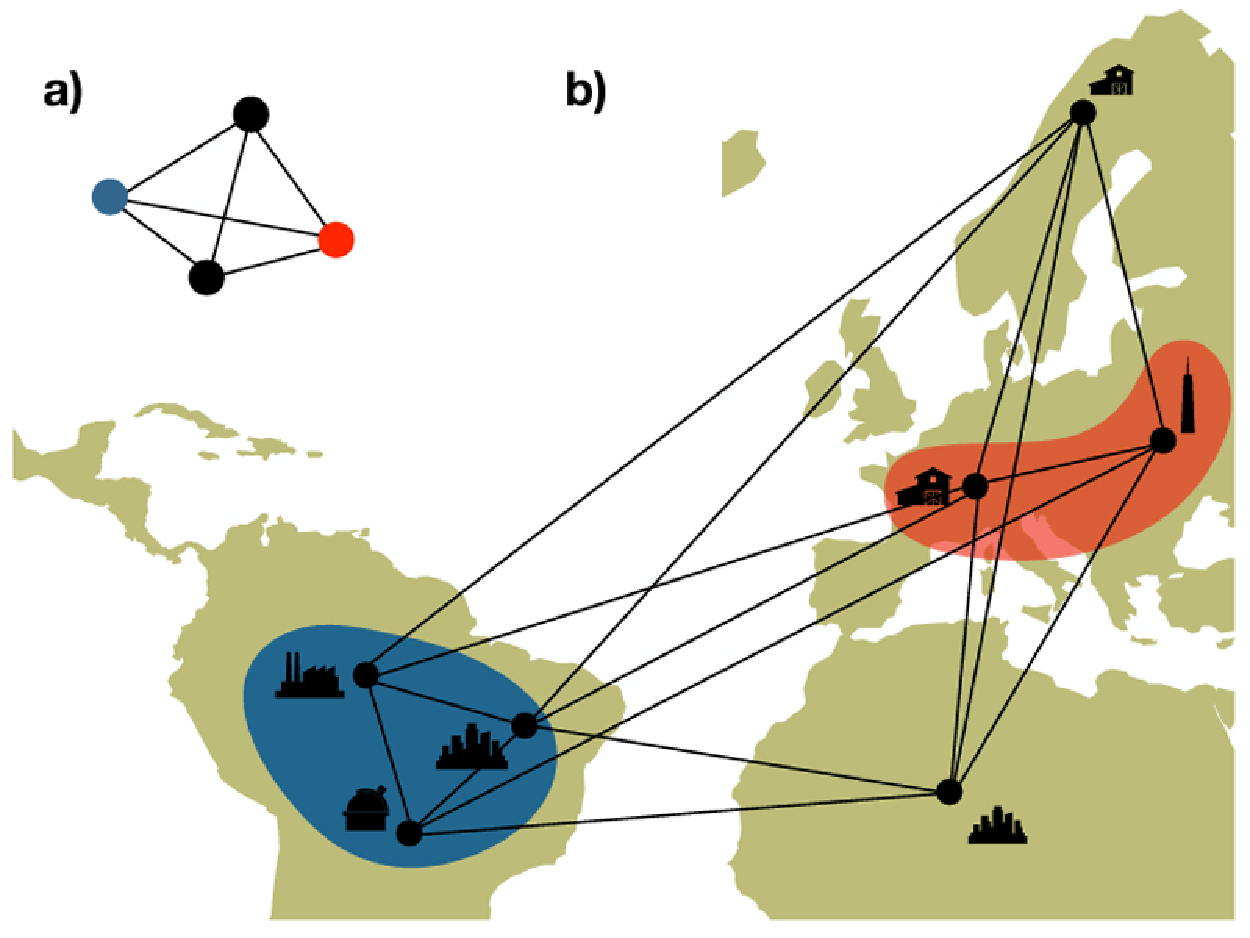
\includegraphics[width=0.65\textwidth]{figures/images/img-1.pdf}
        \caption{\centering a) Effective Quantum Communication Network for self-testing, where each cluster is treated as a single party. b) Corresponding pictorial representation of a quantum network with cooperating clusters. Shaded blue and red regions indicate nodes that are likely to collude.}
    \end{figure}
    
    \noindent of the operations and tasks performed by the quantum nodes or devices in that quantum network. Thus, the main goal of a DI scenario would be for these quantum nodes and devices to perform these operations and tasks only based on statistics of inputs and outputs rather than the exact details of the laboratories of the experimental setup for this designed quantum network.
    
    This seminar addresses aspects of a research work published by Gl\'{a}ucia Murta from Heinrich-Heine University of D\"{u}sseldorf in collaboration with Flavio Baccari from Max-Planck Institute of Quantum Optics, where they introduced a framework for DI entanglement certification with the presence\break of dishonest parties, obtaining some self-testing properties and a robust\break certification of particular resource states such as Greenberger–Horne–Zeilinger (GHZ) states \cite{greenberger-horne-zeilinger:going-beyond-bell-theorem:2007:02-2024} in these Quantum Communication Network scenarios \cite{murta-baccari:self-testing-dishonest-parties-dishonest-parties-device-independent-entanglement-certification-quantum-communication-networks:2023:02-2024}.
    
    \section{Entanglement Certification}
    \label{sec:entanglement-certification}

    The first part of this seminar addressed a simple qualitative overview of the scenario previously introduced, with only an entanglement verification of a simple quantum network. In this simple scenario, instead of having several\break different clusters of collaborating parties, we have only $N$ parties and\break a subset $D$ of $(N - K + 1)$ dishonest parties that could be collaborating. This simple scenario is a little different from the standard DI scenario. Namely, in the DI scenario, we assume we do not know what the quantum devices or nodes are actually doing. On the other hand, in this scenario variant, some of\break those quantum devices or nodes could work together and apply some\break arbitrary joint operations they could communicate. Therefore, in this new scenario, we do not have this overview network separation, and, in fact, we could say one subset of parties is dishonest, although we do not need to know which of them is indeed dishonest. In this quantum communication network,\break
    \vspace{-3ex}
    \begin{figure}[ht]
        \centering
        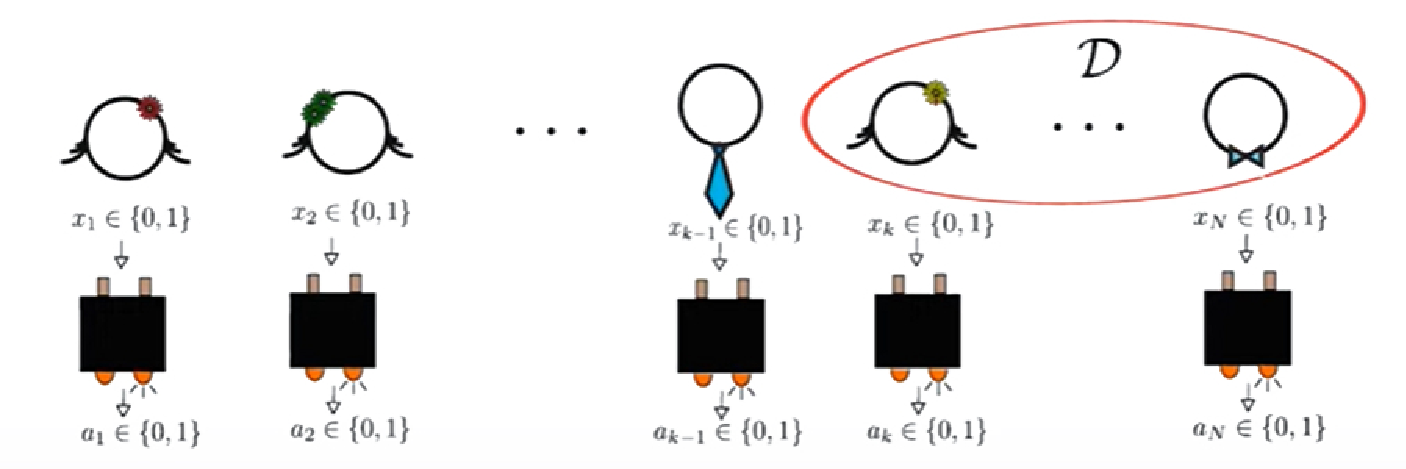
\includegraphics[width=0.8\textwidth]{figures/images/img-2.pdf}
        \caption{\centering Illustration of Quantum Communication Network scenario with\break a set $\mathcal{D}$ of dishonest parties.}
    \end{figure}

    \clearpage
    
    \noindent the honest parties only have local uncharacterized quantum devices or\break quantum nodes. On the other hand, the dishonest ones are allowed to\break communicate among themselves, apply classical post-processing operations, and perform joint measurements. In this scenario, we assume the dishonest parties can also control their quantum devices or quantum nodes. However, in the end, we can obtain the statistics, and therefore, we still want to analyze the distributed quantum entanglements through the quantum network.

    But the crucial aspect here is that we are actually going to address a DI scenario where we will need a Bell Inequality \cite{bell:einstein-podolsky-rosen-paradox:1964:02-2024}. The results obtained by the authors demonstrate we can use a particular class of Bell Inequalities to achieve such a strong characterization for this scenario. In this case, the Bell Inequality of interest is called the Svetlichny Inequality \cite{svetlivhny:distinguishing-three-body-from-two-body-nonseparability-bell-type-inequality:1987:02-2024,seevinck-svetlichny:bell-type-inequalities-partial-separability-particle-systems-and-quantum-mechanical-violations:2002:02-2024}, an inequality where each one of the parties gets two inputs and two outputs. This inequality is also known as the Full Correlator Inequality since we only have terms that involve the expected value of the observables of all the parties together. Basically, this correlator results in $1$ if the parity of the parties' measurement outcomes is $0$ and results in $-1$ if the parity of outcomes is $1$.

    \noindent These $N$-partite Svetlichny Inequalities have the following form below:
    $$ {S}_{N}^{\pm} = \sum_{\vec{x}} {(-1)}^{\frac{{w}_{\vec{x}} \times ({w}_{\vec{x}} \pm 1)}{2}} \left\langle {A}_{{x}_{1}}^{(1)} {A}_{{x}_{2}}^{(2)} \dots {A}_{{x}_{N}}^{(N)} \right\rangle $$
    
    $$ \mathrm{\text{Where:}} $$
    $$ \vec{x} = ({x}_{1}, {x}_{2}, \dots {x}_{N})\mathrm{\text{ is the bitstring of inputs for all $N$ parties,}} $$
    $$ {w}_{\vec{x}}\mathrm{\text{ is the Hamming weight of $\vec{x}$,}} $$
    $$ \left\langle {A}_{{x}_{1}}^{(1)} {A}_{{x}_{2}}^{(2)} \dots {A}_{{x}_{N}}^{(N)} \right\rangle = p\left( {\oplus}_{j=1}^{N} {a}_{j} = 0 | {x}_{1}{x}_{2} \dots {x}_{N} \right) - p\left( {\oplus}_{j=1}^{N} {a}_{j} = 1 | {x}_{1}{x}_{2} \dots {x}_{N} \right)\mathrm{\text{,}} $$
    $$ \mathrm{\text{and }} {S}_{N}^{\pm} \stackrel{\mathcal{C}}{\leq} {2}^{(N - 1)} \stackrel{\mathcal{Q}}{\leq} {2}^{(N - 1)} \times \sqrt{2}\mathrm{\text{,}} $$
    $$ \mathrm{\text{for a classical bound $\mathcal{C}$ and a (estimated) quantum bound $\mathcal{Q}$.}} $$

    \noindent Therefore, this is a family of $N$-partite Svetlichny Inequalities for any number $N$ of parties. Such as any other Bell Inequality, these Svetlichny Inequalities\break have a classical bound that Quantum Mechanics can violate, as well as they have a (estimated) quantum bound. However, this classical bound is a little more interesting in the sense that when we have more than $N = 2$ parties,\break we start having a structure for the outcomes of our parties involved, so we do not have only a separable notion for them (e.g., local or non-local),\break but also a different structure notion, namely a party grouping concept.
    
    \noindent This classical bound ${S}_{N}^{\pm} \stackrel{\mathcal{C}}{\leq} {2}^{(N - 1)}$ sets a limit for all the probability\break distributions in a way we cannot decompose them in the following form:
    \begin{equation*}
        \begin{gathered}
            p({a}_{1} {a}_{2} \dots {a}_{N} | {x}_{1} {x}_{2} \dots {x}_{N}) = \\
            = \sum_{\mathcal{P} \subsetneq [N]} \int p(\lambda) \times \underbrace{p\left({a}_{\mathcal{P}} | ({x}_{\mathcal{P}} \times \lambda)\right)}_{\mathrm{\text{\color{Red} arbitrary \color{Black} \footnotemark}}} \times p\left({a}_{{\mathcal{P}}^{\mathcal{C}}} | ({x}_{{\mathcal{P}}^{\mathcal{C}}} \times \lambda)\right)\ d\lambda
        \end{gathered}
    \end{equation*}
    \footnotetext{Detects \color{Red} strong \color{Black} genuine multipartite non-locality.}
    
    \noindent From this mathematical form, we can divide the subset of parties into two main groups, where we may have arbitrary collaborations within these groups, but we still have some separate actions. Then, we can take some convex combination of this type of correlation, where we have arbitrary\break correlations within these groups of parties. And, since these correlations are within this local classical bound, we are able to witness a strong genuine\break multipartite non-locality. Thus, we violate the Svetlichny Inequality only when we cannot decompose this probability distribution in this mathematical\break form. Nowadays, the first proposal for the definition of genuine multipartite non-locality, where Svetlichny allowed this joint probability distribution of the group to be arbitrary, is not used anymore because when we abstract from the considered scenario, we usually want to look at non-locality property as an operational framework, what leads to some inconsistencies if we define\break locality regarding that operational outlook \cite{gallego-wurflinger-acin-navascues:operational-framework-nonlocality:2012:02-2024}. To overcome this, people often add some assumptions to these joint probability distributions, often assuming\break they have to be non-signaling or one-way signaling \cite{gallego-wurflinger-acin-navascues:operational-framework-nonlocality:2012:02-2024,bancal-barrett-gisin-pironio:definitions-multipartite-nonlocality:2013:02-2024}, but they cannot be\break arbitrary. However, for our scenario, it turns out that this definition is the one that is interesting because we want to address these collaborating parties that could be realizing an arbitrary action. Another important observation is that this inequality also detects Genuine Multipartite Entanglement (GME) since we would never be able to violate it if the quantum entangled state we want to verify is bi-separable in the standard Bell Inequality scenario.

    \noindent A violation of this GME would imply the following mathematical expression:
    $$ \rho \neq \sum_{\mathcal{P} \subsetneq [N]} \sum_{i} {q}_{\mathcal{P}}^{i} \times {\rho}_{\mathcal{P}}^{i} \otimes {\rho}_{{\mathcal{P}}^{\mathcal{C}}}^{i} $$
    
    \noindent For the Svetlichny Inequality with dishonest parties, the honest action would be the following observable, which describes a subtraction between two\break arbitrary Positive Operator-Valued Measure (POVM) elements, one for each measurement outcome, where, in principle, honest actions should apply local actions, but they will have these two global POVM elements instead:
    $$ \mathrm{\text{\color{Cyan}\textbf{Honest Action: }\color{Black} }} {A}_{{x}_{i}}^{(i)} = {\prod}_{0|{x}_{i}} - {\prod}_{1|{x}_{i}} \mathrm{\text{, }} i \in \mathcal{H} $$
    $$ \mathrm{\text{\color{Red}\textbf{Dishonest Action: }\color{Black} }} {A}_{{x}_{K}}^{(K)} \times {A}_{{x}_{(K + 1)}}^{(K + 1)} \times \dots {A}_{{x}_{N}}^{(N)} \rightarrow {M}_{{x}_{K} {x}_{(K + 1)} \dots {x}_{N}}^{(N)} $$

    \noindent Now we can look at the Svetlichny Inequality for $N = 3$ (similar to\break the tripartite Mermin's Inequality \cite{mermin:extreme-quantum-entanglement-superposition-macroscopically-distinct-states:1990:02-2024} that contains half of the terms of this\break tripartite Svetlichny Inequality) through the mathematical expression below:
    $$ N = 3 \mathrm{\text{, }} \mathcal{H} = \{ \mathrm{\text{Alice}} \} \mathrm{\text{, }} \mathcal{D} = \{ \mathrm{\text{Bob, Charlie}} \} $$
    \begin{equation*}
        \begin{aligned}
            {S}_{3} = & \left\langle {A}_{0} {B}_{0} {C}_{0} \right\rangle - \left\langle {A}_{0} {B}_{1} {C}_{0} \right\rangle - \left\langle {A}_{1} {B}_{0} {C}_{0} \right\rangle - \left\langle {A}_{1} {B}_{1} {C}_{0} \right\rangle \\
            & - \left\langle {A}_{0} {B}_{0} {C}_{1} \right\rangle - \left\langle {A}_{0} {B}_{1} {C}_{1} \right\rangle - \left\langle {A}_{1} {B}_{0} {C}_{1} \right\rangle + \left\langle {A}_{1} {B}_{1} {C}_{1} \right\rangle \Leftrightarrow
        \end{aligned}
    \end{equation*}
    \begin{equation*}
        \begin{aligned}
            {S}_{3} = & \left\langle {A}_{0} {M}_{00} \right\rangle - \left\langle {A}_{0} {M}_{10} \right\rangle - \left\langle {A}_{1} {M}_{00} \right\rangle - \left\langle {A}_{1} {M}_{10} \right\rangle \\
            & - \left\langle {A}_{0} {M}_{01} \right\rangle - \left\langle {A}_{0} {M}_{11} \right\rangle - \left\langle {A}_{1} {M}_{01} \right\rangle + \left\langle {A}_{1} {M}_{11} \right\rangle
        \end{aligned}
    \end{equation*}
    
    \noindent Thus, this Svetlichny Inequality contains all the possible terms we might have, and we can recall that Quantum Mechanics does not saturate the\break algebraic bound in this inequality. For example, for a tripartite scenario, we can have Alice as an honest party, while Bob and Charlie are dishonest\break parties. Therefore, Bob and Charlie can apply a joint operator, and we can rebuild what is the actual inequality with the mathematical expression below:
    \begin{equation*}
        \begin{aligned}
            {S}_{3} = & \color{Cyan}\left\langle {A}_{0} {M}_{00} \right\rangle - \left\langle {A}_{0} {M}_{10} \right\rangle - \left\langle {A}_{1} {M}_{00} \right\rangle - \left\langle {A}_{1} {M}_{10} \right\rangle \\
            & \color{Red} - \left\langle {A}_{0} {M}_{01} \right\rangle - \left\langle {A}_{0} {M}_{11} \right\rangle - \left\langle {A}_{1} {M}_{01} \right\rangle + \left\langle {A}_{1} {M}_{11} \right\rangle \\
            = & \color{Cyan} {\beta}_{0} \color{Black} + \color{Red} {\beta}_{1}
        \end{aligned}
    \end{equation*}
    $$ \Downarrow $$
    $$ {S}_{3} \leq 2 \times \max{ \{ {\beta}_{0}, {\beta}_{1} \} } = 2 \times \beta, \color{Red} \beta \geq \frac{{S}_{3}}{2} \color{Black} $$
    
    \noindent By doing this mathematical reformulation, if we are familiar with\break the non-locality concept, we can recognize two Clauser-Horne-Shimony-Holt (CHSH) Inequalities in the expression resulting from it. The structure of these symmetric Svetlichny Inequalities says that if we have a tripartite\break inequality and violate it with these dishonest parties, we know they are in a Bell scenario with two practical parties. On one side, we have Alice as an honest party from set $\mathcal{H}$, and on the other, we have Bob and Charlie together in a group from set $\mathcal{D}$, and they would be violating the CHSH Inequality.

    \noindent What we show is that this property happens for any number $K$ of honest\break parties and any total number $N$ of parties. So, whenever we have Svetlichny Inequality and $K$ effective parties, we would have a violation of a\break corresponding $K$-partite inequality in the standard Bell scenario, where these $K$ parties are not communicating. Thus, we have the following statement:
    $$ |\mathcal{H}| = (K - 1)\mathrm{\text{, }} |\mathcal{D}| = (N - K + 1) $$
    $$ \mathrm{\text{Violation of ${S}_{N}$ in the Svetlichny Inequality Scenario}} $$
    $$ \Downarrow $$
    $$ \mathrm{\text{Violation of ${S}_{K}$ in the standard Bell Inequality Scenario}} $$
    $$ \mathrm{\text{With:}} $$
    $$ \color{Red} {S}_{K} \geq \frac{{S}_{N}}{{2}^{(N - K)}} \color{black}\mathrm{\text{,}} $$
    $$ \mathrm{\text{where ${S}_{N}$ denotes violation of ${S}_{N}^{+}$ or ${S}_{N}^{-}$.}} $$
    
    \noindent From this property, we can get this qualitative certification where we do\break not know which parties in our Quantum Communication Network are\break dishonest, but we are certifying that we have a genuine $K$-partite quantum\break entanglement between the sets of honest parties and dishonest parties. As a result, we obtain a \textbf{certification of \color{Red}genuine $K$-partite entanglement \color{Black} among the honest parties and the unknown set of dishonest parties}.
    
    
    \section{Self-Testing with Dishonest Parties}
    \label{sec:self-testing-with-dishonest-parties}

    In particular, what is interesting here is that we can also perform\break a stronger characterization of our simplest scenario, such that we do not have just the qualitative entanglement witnessing but also a self-testing result in that scenario. For completeness and to define this self-testing, we should\break consider that we have a probability distribution of outcomes given the inputs,\break and with that, we can infer that we have a specific quantum state. Namely, all the self-testing results cannot guarantee the absolute occurrence of this quantum state. However, we can infer its occurrence from the correlations of the probability distribution of outcomes up to some undetectable symmetry (local isometries), and we can be sure that we have our quantum state $|\phi\rangle$. Then, the formal self-testing statement will be of the following form:
    $$ p({a}_{1}, {a}_{2}, \dots, {a}_{N}|{x}_{1}, {x}_{2}, \dots, {x}_{N}) \longrightarrow |\phi\rangle\footnotemark $$
    $$ \mathrm{\text{From which it is stated the following:}} $$
    $$ {\Lambda}_{1} \otimes {\Lambda}_{2} \otimes \dots \otimes {\Lambda}_{N} (|\psi\rangle) = |\phi\rangle \otimes |\zeta\rangle \mathrm{\text{,}} $$
    $$ \mathrm{\text{where:}} $$
    $$ \mathrm{\text{$|\psi\rangle$: Quantum state producing the observed correlations,}} $$
    $$ \mathrm{\text{$|\zeta\rangle$: Uncorrelated degrees of freedom, and}} $$
    $$ \mathrm{\text{${\Lambda}_{i}$: Local isometries.}} $$
    \footnotetext{Up to undetectable symmetries (local isometries).}
    
    \noindent We have a quantum state $|\psi\rangle$ that produces the correlations we observed, and these correlations ensure that there is a set of local isometries ${\Lambda}_{i}$, with $1 \leq i \leq N$, that we could apply to the quantum state that brings me to the target quantum state $|\phi\rangle$ and some extra uncorrelated degrees of freedom $|\zeta\rangle$.

    \noindent Now, we can extend this definition of self-testing to the DI quantum network scenario. Here, the idea is that we cannot prevent the set of dishonest parties from applying a global operation. So, we would define the self-testing up to local isometries and global isometry of the set of dishonest parties. Moreover, the authors proved that if we have the maximum violation of this Svetlichny Inequality, we could self-test that we have the $K$-partite GHZ state between the set of honest parties and the global set of dishonest parties. Therefore, \textbf{a maximum violation of an $N$-partite Svetlichny Inequality \color{Red} self-tests a $K$-partite GHZ state \color{Black} shared by the honest parties and the set of dishonest parties $\mathcal{D}$}, as we mathematically demonstrate below:
    $$ {\Lambda}_{1} \otimes {\Lambda}_{2} \otimes \dots \otimes {\Lambda}_{(K - 1)} \otimes {\Lambda}_{\mathcal{D}} (|\psi\rangle) = \left| {\phi}_{GHZ}^{K} \right\rangle \otimes |\zeta\rangle $$

    \clearpage
    
    \noindent In order to give a little idea of the corresponding proof, let's consider the previously mentioned observation that there are some CHSH Inequalities\break in the Svetlichny Inequality. Namely, the Svetlichny Inequality has several terms that increase with the number $N$ of parties. But, we can always decompose this inequality into some inequalities called ${S}_{2}$, for example. We use this terminology because the first and the second parties have different inputs, but all the other parties have the same fixed input. Thus, the first and second parties provide a CHSH Inequality, while the remaining parties always provide the same input for the mathematical expressions below:
    \begin{equation*}
        \begin{aligned}
            {S}_{N}^{+} & = \sum_{\stackrel{{\vec{x}}_{(N - 2)}}{{\omega}_{\vec{x}}\mathrm{\text{ odd}}}} {(-1)}^{\frac{ {\omega}_{{\vec{x}}_{(N - 2)}} \cdot \left( {\omega}_{{\vec{x}}_{(N - 2)}} + 1 \right) }{2}} \times {S}_{2}^{-} \times \left( {\vec{x}_{(N - 2)}} \right) + \\
            & + \sum_{\stackrel{{\vec{x}}_{(N - 2)}}{{\omega}_{\vec{x}}\mathrm{\text{ even}}}} {(-1)}^{\frac{ {\omega}_{{\vec{x}}_{(N - 2)}} \cdot \left( {\omega}_{{\vec{x}}_{(N - 2)}} + 1 \right) }{2}} \times {S}_{2}^{+} \times \left( {\vec{x}_{(N - 2)}} \right)
        \end{aligned}
    \end{equation*}
    $$ \mathrm{\text{Where:}} $$
    \begin{equation*}
        \begin{aligned}
            {S}_{2}^{+} \left( {\vec{x}_{(N - 2)}} \right) & = \left\langle \color{Red} {A}_{0}^{(1)} {A}_{0}^{(2)} \color{Black} {A}_{{x}_{3}}^{(3)} \dots {M}_{{\vec{x}}_{\mathcal{D}}}^{(K)} \right\rangle - \left\langle \color{Red} {A}_{0}^{(1)} {A}_{1}^{(2)} \color{Black} {A}_{{x}_{3}}^{(3)} \dots {M}_{{\vec{x}}_{\mathcal{D}}}^{(K)} \right\rangle - \\
            & - \left\langle \color{Red} {A}_{1}^{(1)} {A}_{0}^{(2)} \color{Black} {A}_{{x}_{3}}^{(3)} \dots {M}_{{\vec{x}}_{\mathcal{D}}}^{(K)} \right\rangle - \left\langle \color{Red} {A}_{1}^{(1)} {A}_{1}^{(2)} \color{Black} {A}_{{x}_{3}}^{(3)} \dots {M}_{{\vec{x}}_{\mathcal{D}}}^{(K)} \right\rangle
        \end{aligned}
    \end{equation*}
    \begin{equation*}
        \begin{aligned}
            {S}_{2}^{-} \left( {\vec{x}_{(N - 2)}} \right) & = \left\langle \color{Red} {A}_{0}^{(1)} {A}_{0}^{(2)} \color{Black} {A}_{{x}_{3}}^{(3)} \dots {M}_{{\vec{x}}_{\mathcal{D}}}^{(K)} \right\rangle + \left\langle \color{Red} {A}_{0}^{(1)} {A}_{1}^{(2)} \color{Black} {A}_{{x}_{3}}^{(3)} \dots {M}_{{\vec{x}}_{\mathcal{D}}}^{(K)} \right\rangle + \\
            & + \left\langle \color{Red} {A}_{1}^{(1)} {A}_{0}^{(2)} \color{Black} {A}_{{x}_{3}}^{(3)} \dots {M}_{{\vec{x}}_{\mathcal{D}}}^{(K)} \right\rangle - \left\langle \color{Red} {A}_{1}^{(1)} {A}_{1}^{(2)} \color{Black} {A}_{{x}_{3}}^{(3)} \dots {M}_{{\vec{x}}_{\mathcal{D}}}^{(K)} \right\rangle
        \end{aligned}
    \end{equation*}
    
    \noindent Another part of the proof idea is that these ${S}_{2}$ Inequalities are very similar to CHSH Inequalities, except we have the operators of all the other parties. Then, we can construct a Sum Of Squares (SOS) decomposition of each term, which is usually a standard technique used to prove self-testing experimental\break\clearpage\noindent results. This SOS decomposition for each term is demonstrated below:
    \begin{equation*}
        \begin{aligned}
            2 \times \sqrt{2} \times \mathds{1} - {\hat{S}}_{2,{\vec{x}_{(N - 2)}} }^{+} = \frac{1}{\sqrt{2}} & \left[ {\left( \mathds{1} - \frac{{\hat{A}}_{0}^{(1)} - {\hat{A}}_{1}^{(1)}}{\sqrt{2}} {\hat{A}}_{0}^{(2)} \dots {A}_{{x}_{(K - 1)}}^{(K - 1)} {M}_{{\vec{x}}_{\mathcal{D}}}^{(K)} \right)}^{2} + \right. \\
            & \left. \hspace{-0.5ex} + {\left( \mathds{1} + \frac{{\hat{A}}_{0}^{(1)} + {\hat{A}}_{1}^{(1)}}{\sqrt{2}} {\hat{A}}_{1}^{(2)} \dots {A}_{{x}_{(K - 1)}}^{(K - 1)} {M}_{{\vec{x}}_{\mathcal{D}}}^{(K)} \right)}^{2} \right]
        \end{aligned}
    \end{equation*}
    \begin{equation*}
        \begin{aligned}
            2 \times \sqrt{2} \times \mathds{1} - {\hat{S}}_{2,{\vec{x}_{(N - 2)}} }^{-} = \frac{1}{\sqrt{2}} & \left[ {\left( \mathds{1} - \frac{{\hat{A}}_{0}^{(1)} + {\hat{A}}_{1}^{(1)}}{\sqrt{2}} {\hat{A}}_{0}^{(2)} \dots {A}_{{x}_{(K - 1)}}^{(K - 1)} {M}_{{\vec{x}}_{\mathcal{D}}}^{(K)} \right)}^{2} + \right. \\
            & \left. \hspace{-0.5ex} + {\left( \mathds{1} - \frac{{\hat{A}}_{0}^{(1)} - {\hat{A}}_{1}^{(1)}}{\sqrt{2}} {\hat{A}}_{1}^{(2)} \dots {A}_{{x}_{(K - 1)}}^{(K - 1)} {M}_{{\vec{x}}_{\mathcal{D}}}^{(K)} \right)}^{2} \right]
        \end{aligned}
    \end{equation*}
    
    \noindent Then, we can finally obtain the stabilizer conditions, as well as the\break respective commutation relations of the operator for a $K$-partite GHZ state:
    \begin{equation*}
        \begin{gathered}
           {(-1)}^{\frac{ {\omega}_{{\vec{x}}_{(N - 2)}} \cdot \left( {\omega}_{{\vec{x}}_{(N - 2)}} + 1 \right) }{2}} \times \frac{{A}_{0}^{(1)} + {A}_{1}^{(1)}}{\sqrt{2}} \times {A}_{0}^{(2)} \dots {A}_{{x}_{(K - 1)}}^{(K - 1)} {M}_{{\vec{x}}_{\mathcal{D}}}^{(K)} |\psi\rangle = |\psi\rangle \mathrm{\text{,}} \\
           \mathrm{\text{with }} {\omega}_{{\vec{x}_{(N - 2)}}} \mathrm{\text{ odd,}}
        \end{gathered}
    \end{equation*}
    \begin{equation*}
        \begin{gathered}
           {(-1)}^{\frac{ {\omega}_{{\vec{x}}_{(N - 2)}} \cdot \left( {\omega}_{{\vec{x}}_{(N - 2)}} + 1 \right) }{2}} \times \frac{{A}_{0}^{(1)} - {A}_{1}^{(1)}}{\sqrt{2}} \times {A}_{1}^{(2)} \dots {A}_{{x}_{(K - 1)}}^{(K - 1)} {M}_{{\vec{x}}_{\mathcal{D}}}^{(K)} |\psi\rangle = |\psi\rangle \mathrm{\text{,}} \\
           \mathrm{\text{with }} {\omega}_{{\vec{x}_{(N - 2)}}} \mathrm{\text{ odd,}}
        \end{gathered}
    \end{equation*}
    \begin{equation*}
        \begin{gathered}
           {(-1)}^{\frac{ {\omega}_{{\vec{x}}_{(N - 2)}} \cdot \left( {\omega}_{{\vec{x}}_{(N - 2)}} + 1 \right) }{2}} \times \frac{{A}_{0}^{(1)} - {A}_{1}^{(1)}}{\sqrt{2}} \times {A}_{0}^{(2)} \dots {A}_{{x}_{(K - 1)}}^{(K - 1)} {M}_{{\vec{x}}_{\mathcal{D}}}^{(K)} |\psi\rangle = |\psi\rangle \mathrm{\text{,}} \\
           \mathrm{\text{with }} {\omega}_{{\vec{x}_{(N - 2)}}} \mathrm{\text{ even, and}}
        \end{gathered}
    \end{equation*}
    \begin{equation*}
        \begin{gathered}
           {(-1)}^{\frac{ {\omega}_{{\vec{x}}_{(N - 2)}} \cdot \left( {\omega}_{{\vec{x}}_{(N - 2)}} + 1 \right) }{2}} \times \frac{{A}_{0}^{(1)} + {A}_{1}^{(1)}}{\sqrt{2}} \times {A}_{1}^{(2)} \dots {A}_{{x}_{(K - 1)}}^{(K - 1)} {M}_{{\vec{x}}_{\mathcal{D}}}^{(K)} |\psi\rangle = |\psi\rangle \mathrm{\text{,}} \\
           \mathrm{\text{with }} {\omega}_{{\vec{x}_{(N - 2)}}} \mathrm{\text{ even.}}
        \end{gathered}
    \end{equation*}

    \noindent In particular, the authors showed an experimental result we do not know so far. Namely, we cannot only use the Mermin's Inequality to self-test the GHZ state, but we can also use the Svetlichny Inequality for that purpose.

    \noindent Thus, in self-testing, we want to infer if we have the maximum violation and the exact GHZ state. In order to build realistic quantum cryptographic protocols that we can implement shortly, the authors tried to make some robust statements about the quantum state obtained when we do not have a maximum violation of the entanglement. In that direction, for the second part of the proof, the authors tried to deduce which privacy guarantees we can have as a mathematical function of this maximum violation. For that, the authors introduced the concept of fidelity with the target quantum state, generalizing what happens for the standard Bell scenario. In this case, let's assume we have an arbitrary quantum state $\rho$, and we want to see what fidelity we can obtain for the expected N-partite GHZ state, up to the local quantum channels ${\Lambda}_{i}$ and global quantum channel ${\Lambda}_{D}$, with the dishonest parties. We can make this statement because, ideally, we would expect the Quantum Communication Network to distribute this $N$-partite GHZ state. However, it can be distributing another arbitrary quantum state, and we are giving the freedom to the set of dishonest parties to act in that network. So, we can define this described self-testing scenario mathematically as follows:
    $$ {\mathcal{F}}_{DI}^{\mathcal{D} ({S}_{N})} = \inf_{\rho \in \mathcal{S} \left( {S}_{N}^{\mathcal{D}} \right) } \max_{{\Lambda}_{\mathcal{D}}, {\{ {\Lambda}_{i} \}}_{i \in \mathcal{H}} } \mathcal{F}\left( {\otimes}_{i \in \mathcal{H}}\ {\Lambda}_{i} \otimes {\Lambda}_{\mathcal{D}} ( \rho ), {\phi}_{GHZ}^{N} \right) $$
    $$ \mathrm{\text{Where:}} $$
    $$ \mathrm{\text{\color{Cyan} \textbf{$\mathcal{S}( {S}_{N}^{\mathcal{D}} )$:} \color{Black} Quantum States that achieve value ${S}_{N}$ with dishonest parties $\mathcal{D}$; }} $$
    $$ \mathrm{\text{\color{Cyan} \textbf{${\Lambda}_{i}$:} \color{Black} Local Quantum Communication Channels, with $1 \leq i \leq N$; }} $$
    $$ \mathrm{\text{\color{Cyan} \textbf{${\Lambda}_{i}$:} \color{Black} Global Quantum Communication Channel with dishonest parties $\mathcal{D}$. }} $$
    
    
    \noindent In the standard Bell scenario, and regarding this self-testing quantity, we do not have the freedom of operations for the set of dishonest parties.\break However, J\c{e}drzej Kaniewski introduced this self-testing quantity before, and he also introduced a method to bound the fidelity in the standard Bell\break scenario, called Self-Testing from the OPerator Inequalities (STOPI) \cite{kaniewski:analytic-nearly-optimal-self-testing-bounds-clauser-horne-shimony-holt-and-mermin-inequalities:2016:02-2024,coopmans-kaniewski-schaffner:robust-self-testing-two-qubit-states:2019:02-2024}. This method transforms the fidelity we pretend to bound into an operator\break inequality and then calculates some coefficients for this fidelity bound. Some\break further research work on this concept was done by J\c{e}drzej Kaniewski, Tim\break Coopmans, and Christian Schaffner, namely in explaining better this method and using it for different Bell Inequalities. For what remains of the idea proof, the authors also showed that in the case we want to bound the fidelity of our quantum state in the presence of dishonest parties, if we have a fixed number $N - K + 1$ of dishonest parties (and $K - 1$ honest parties), such that effectively\break we have a $K$-partite Bell scenario, we can bound this fidelity quantity using\break the same coefficients of the standard $K$-partite Bell scenario. Namely, we only have to apply this method developed for the specific case of the Svetlichny Inequality, and then, we can also generate bounds for the fidelity. We can mathematically define this bound obtained from the STOPI method as:
    $$ {F}_{DI}^{|\mathcal{D}| = (N - K + 1)} \geq {f}_{K} \times \frac{{S}_{N}}{{2}^{(N - K)}} - {\mu}_{K} $$
    $$ \mathrm{\text{Where:}} $$
    $$ {f}_{K} \mathrm{\text{ and }} {\mu}_{K} \mathrm{\text{ are obtained from the STOPI method. }} $$
    \vspace{-1.75ex}
    $$ \mathrm{\text{\textbf{Self-Testing from the OPerator Inequalities (STOPI):}}} $$
    \begin{equation*}
        \begin{aligned}
            \mathcal{F}\left( {\otimes}_{i = 1}^{k}\ {\Lambda}_{i}(\rho), {\phi}_{GHZ}^{K} \right) & = Tr\left( {\otimes}_{i = 1}^{k}\ {\Lambda}_{i}^{\dagger} \left( {\phi}_{GHZ}^{K} \right) \times \rho \right) = \\
            & = Tr(K \times \rho) \rightarrow K - {f}_{K} \times {S}_{K} + {\mu}_{K} \times \mathds{1} \geq 0
        \end{aligned}
    \end{equation*}

    \noindent Thus, we can guarantee that any fidelity value above $50\%$ certainly implies the occurrence of quantum entanglement, but we can also deduce more about the fidelity quantity even when we do not have the maximum violation.
    \vspace{-3ex}
    \begin{figure}[ht]
        \centering
        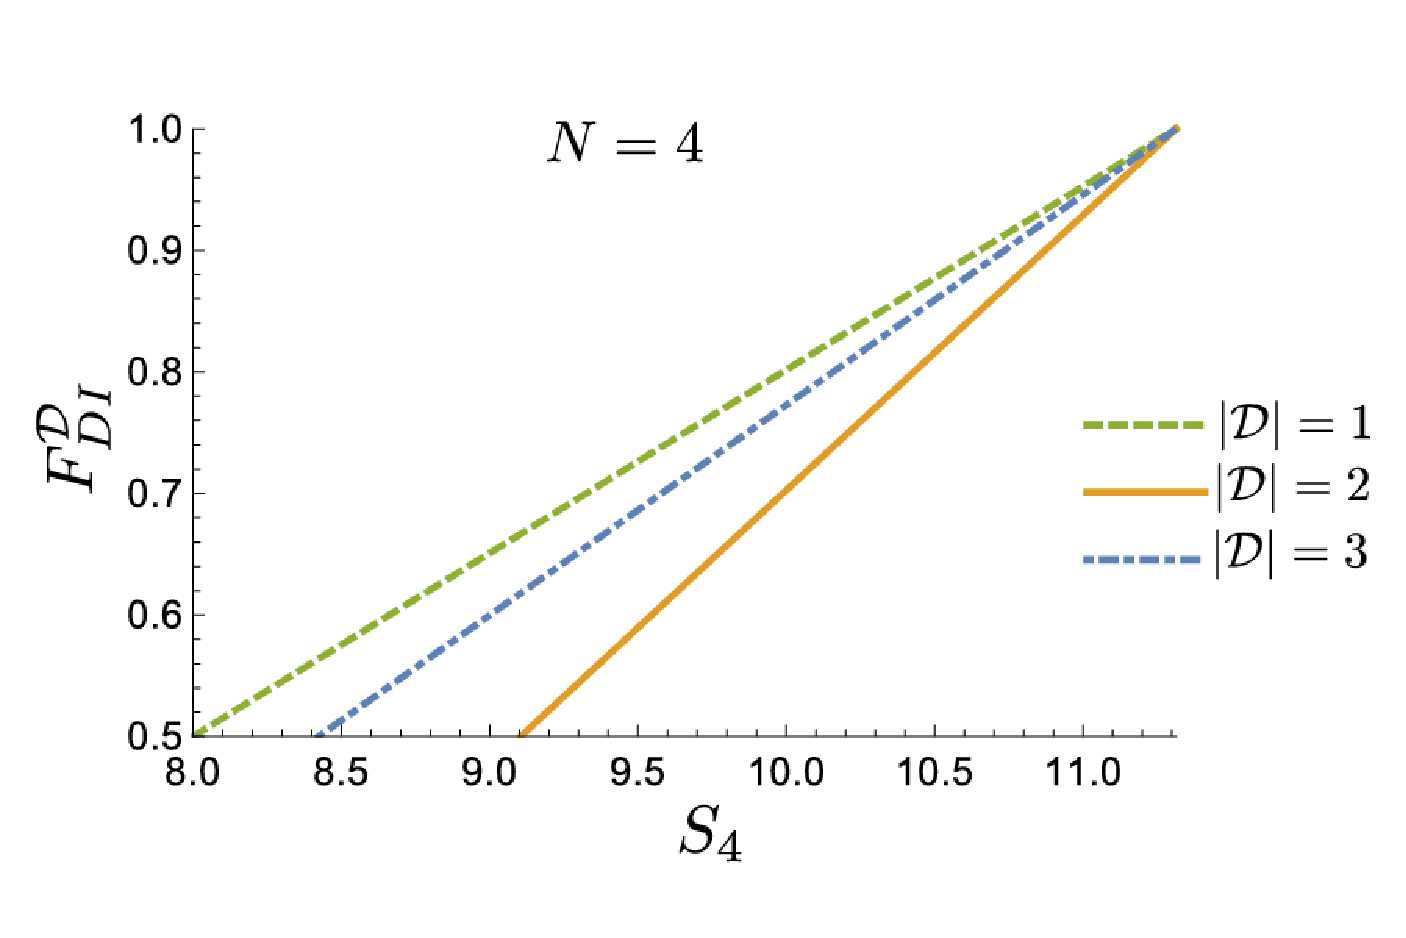
\includegraphics[width=0.65\textwidth]{figures/images/img-3.pdf}
        \vspace{-3.5ex}
        \caption{\centering Numerical lower bounds on the fidelity as a function of the violation of a 4-partite Svetlichny Inequality. The curves represent scenarios with different numbers of dishonest parties.}
    \end{figure}

    \clearpage
    
    \section{Outlook}
    \label{sec:outlook}

    Now, we can think a little more about open questions of the experimental\break results obtained by the author, connecting to Quantum Cryptography. There are many quantum cryptographic protocols where the parties might be\break interested in collaborating and trying to obtain some information before the end of the protocol. Namely, two examples of this situation are the Secret Sharing (SS) and Anonymous Communication protocols. In the SS protocol, a party (e.g., Alice) wants to share a secret (e.g., a quantum or a classical state) with other parties (e.g., Bobs) such that they can recover the secret only if every party collaborates. However, some malicious parties could try to spoil this protocol and get the information before its end. In the Anonymous\break Communication protocol, a sender (e.g., Alice or an abstract $S$) who would like to send a message (e.g., a set of quantum or classical states) to a receiver (e.g., Bob or an abstract $R$) in such a way that everyone in the quantum network has to collaborate for that, but in the end, no one is aware of the identity of each other. Thus, in the end, no one is aware of who is sending the message, and maybe neither the receiver is aware of who sent the message. Therefore, in both of these quantum cryptographic protocols, everyone needs to perform some specific actions, and these protocols are usually based on very particular quantum or classical states to guarantee their security.

    \vspace{-2ex}
    \begin{figure}[ht]
        \centering
        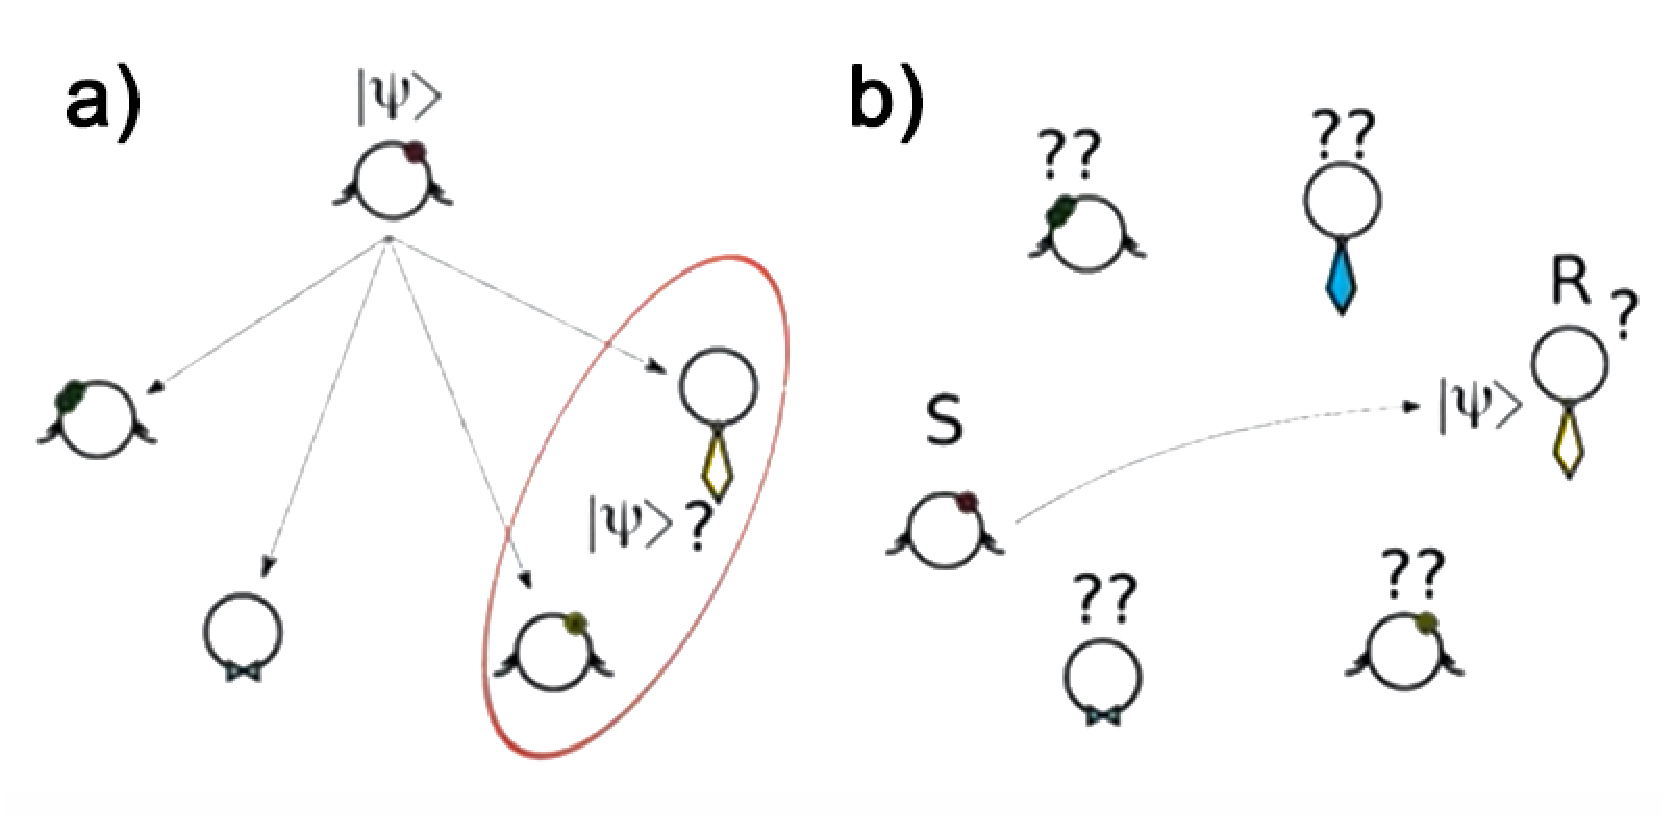
\includegraphics[width=0.6\textwidth]{figures/images/img-4.pdf}
        \vspace{-3.5ex}
        \caption{\centering a) Secret Sharing (SS) protocol.\break b) Anonymous Communication protocol.}
    \end{figure}

    \noindent As a next step, the authors pointed out it is desirable to use these\break experimental results obtained for state certification to prove the security of\break the quantum cryptographic protocols previously mentioned. However, just the certification is not enough to prove it. For example, in the case of the Anonymous Communication protocol, Matthias Christandl and Stephanie Wehner introduced another protocol that uses the GHZ state, and we can\break perform the task of Anonymous Communication once we have that GHZ state, assuming that it is a trusted source that distributes it \cite{christandl-wehner:quantum-anonymous-transmissions:2005:02-2024}. Then, in the\break Anonymous Communication protocol based on this auxiliary protocol, we would like to know that it is the source that distributes the GHZ state but can exist some dishonest parties that might not be following the verification\break protocol correctly. These certification protocols for the GHZ state in the standard DI scenario, where we know which measurements the parties are performing, have been introduced before \cite{unnikrishnan-macfarlane-yi-diamanti-markham-kerenidis:anonymity-practical-quantum-networks:2019:02-2024}. This type of guarantee stating the distance of the quantum state up to a general quantum communication\break channel on the dishonest parties should be ${\Lambda}_{D}
    $ for consistent entropy.\break However, since the distance from the quantum state obtained to the actual\break GHZ state up to local general operations on the dishonest parties is very small, it is enough to guarantee the security of this task of Anonymous\break Communication. Hence, we can use this state certification result to have these security guarantees even when we do not have characterized devices. Thus, for a Device-Dependent (DD) certification of a GHZ state, we can compute the $\epsilon$-security bound in the presence of dishonest parties as follows:
    $$ \min_{{\mathcal{M}}_{\mathcal{D}}} D\left( {Id}_{\mathcal{H}} \otimes {\mathcal{M}}_{\mathcal{D}}(\rho), {\phi}_{GHZ}^{N} \right) \leq \epsilon $$

    \noindent Still addressing the connection between state certification and the task of Anonymous Communication, we have another protocol variant based on the W state \cite{dur-vidal-cirac:three-qubits-entangled-two-inequivalent-ways:2000:02-2024} rather than the GHZ state \cite{lipinska-murta-wehner:anonymous-transmission-noisy-quantum-network-using-w-state:2018:02-2024}. So far, there is no state\break certification for the W state, and maybe the DI scenario approach would be a way to define a non-stabilizer state certification, which we can use to lift the security of this protocol, such that we do not have to trust the source.

    Finally, the type of guarantees \cite{christandl-wehner:quantum-anonymous-transmissions:2005:02-2024} we usually obtain from self-testing is\break insufficient \cite{grasselli-murta-de-jong-hahn-bruss-kampermann-pappa:secure-anonymous-conferencing-quantum-networks:2022:02-2024} because the distance between the quantum state we got and the desired GHZ state is equivalent to the $\epsilon$-security obtained on the protocol\break proposed by the author. For example, for Quantum Key Distribution (QKD) protocols, we can tolerate noise values usually between 10\% and 20\% and have $\epsilon$-security with an $\epsilon$ value as small as we would like just by performing more rounds of the protocols. A big open question is how to use this type of self-testing result more effectively in Quantum Cryptography or even how we apply it to prove the security of these quantum cryptographic protocols, such that we have $\epsilon$-security but also tolerate a reasonable amount of noise.
    
    
    \bibliographystyle{unsrt}

    \clearpage
    
    \bibliography{bibliography}
    \label{bib:bibliography}
    
\end{document}